\documentclass[12pt, aspectratio=169]{beamer}

\input{../header}
\usepackage{booktabs}
\usepackage{tikz}
\usetikzlibrary{patterns}


\title{Probability}
\author{Md. Aminul Islam Shazid}
\date{}


\begin{document}
    {
		\setbeamertemplate{footline}{}    % NO FOOTLINE FOR THESE TWO FRAMES
		\addtocounter{framenumber}{-2}    % not counting the title page and the outline in frame numbers

		\begin{frame}
			\titlepage
		\end{frame}

		\begin{frame}{Outline}
            \vfill
			\tableofcontents[subsectionstyle=hide]
            \vfill
		\end{frame}
	}

	\section{Introduction}

    \begin{frame}{What is Probability?}
        Probability deals with uncertainty and quantifies how likely an event is to occur.
		\begin{itemize}
			\item Many real-life situations involve uncertainty rather than certainty
			\item Probability helps us make informed decisions under uncertainty
			\item It provides a numerical measure of chance, between 0 and 1
			\item A probability close to 0 indicates a rare event
			\item A probability close to 1 indicates a highly likely event
		\end{itemize}
    \end{frame}


	\begin{frame}{Examples}
		Probability concepts appear naturally in daily activities.
		\begin{itemize}
			\item Weather forecasting: chance of rain tomorrow
			\item Medical testing: likelihood that a test result is correct
			\item Games and sports: chances of winning or losing
			\item Traffic planning: probability of congestion at a given time
			\item Finance: risk assessment and expected returns
		\end{itemize}
	\end{frame}


	\begin{frame}{Example: Tossing a Coin}
		\begin{itemize}
			\item The experiment consists of tossing a fair coin once
			\item Possible outcomes are Head (H) and Tail (T)
			\item Each outcome has an equal chance of occurring
			\item Probability of Head = $0.5$
			\item Probability of Tail = $0.5$
		\end{itemize}
	\end{frame}


	\section{Key Concept and Terms}

	\begin{frame}{Basic Principal of Counting}
		\begin{itemize}
			\item If an event can occur in $m$ possible ways and for each of the $m$ possible ways that the first event can occur, there are $n$ possible ways that a second event can occur, then there are in total $m \times n$ possible ways that the two events can occur together
			\item For example, if a person can go from place A to place B in three possible ways, and B to C in two ways, then there are a total of six ways to go from A to C
		\end{itemize}
	\end{frame}


	\begin{frame}{Generalized Basic Principle of Counting}
		\begin{itemize}
			\item If an event can occur in $𝑚_1$ possible ways and for each of the possible ways that the first event can occur, there are $𝑚_2$ possible ways that a second event can occur, and again for each of the $𝑚_1 \times 𝑚_2$ possible ways that the first two events can occur, there are $𝑚_3$ possible ways that a third event can occur, and so on, then there are in total $m_1 \times m_2 \times m_3...$ possible ways that all these events can occur together
		\end{itemize}
	\end{frame}

	\begin{frame}{Permutation}
		A permutation is an arrangement of objects where the order matters.
		\begin{itemize}
			\item Number of permutations of $r$ objects chosen from $n$ distinct objects:
			\[
				^nP_r = \frac{n!}{(n-r)!}
			\]
			\item Used when positions or order are important
			\item Example:
			\begin{itemize}
				\item Number of ways to arrange 3 students out of 5 in a row:
				\[
					^5P_3 = \frac{5!}{2!} = 60
				\]
			\end{itemize}
		\end{itemize}
	\end{frame}


	\begin{frame}{Combination}
	A combination is a selection of objects where the order does not matter.
		\begin{itemize}
			\item Number of combinations of $r$ objects chosen from $n$ distinct objects:
			\[
				^nC_r = \frac{n!}{r!(n-r)!}
			\]
			\item Used when only selection matters, not arrangement
			\item Example:
			\begin{itemize}
				\item Number of ways to choose 3 students from 5:
				\[
					^5C_3 = \frac{5!}{3!2!} = 10
				\]
			\end{itemize}
		\end{itemize}
	\end{frame}


	\begin{frame}{Experiment}
		\begin{itemize}
			\item An experiment is any process that can be repeated under certain conditions and that produces an observable result
			\item The result of an experiment is called an outcome
			\item Example:
			\begin{itemize}
				\item Tossing a coin or a dice
				\item Measuring daily rainfall
				\item Conducting chemical reactions
			\end{itemize}
		\end{itemize}		
	\end{frame}


	\begin{frame}{Outcome}
		\begin{itemize}
			\item An outcome is a single possible result of an experiment
			\item There can be one or more \emph{potential} outcomes
			\item Each experiment produces exactly one outcome
			\item Outcomes may be numerical or categorical
			\item Example:
			\begin{itemize}
				\item Getting a head when tossing a coin
				\item Getting a 4 when throwing a dice
			\end{itemize}
		\end{itemize}		
	\end{frame}


	\begin{frame}{Types of Experiment}
		Experiments can be categorized in to two types based on the nature of their outcome(s):
		\begin{itemize}
			\item Deterministic: outcome is known or can be predicted with certainty
			\item Random: outcome is unknown and cannot be predicted with certainty
		\end{itemize}
	\end{frame}


	\begin{frame}{Random Experiment}
	A random experiment is an experiment whose outcome cannot be predicted with certainty.
		\begin{itemize}
			\item The same experiment may produce different outcomes on repetition
			\item Potential outcomes are known, but which one will occur is uncertain
			\item Examples:
			\begin{itemize}
				\item Tossing a coin
				\item Rolling a dice
				\item Drawing a card from a shuffled deck
			\end{itemize}
		\end{itemize}
	\end{frame}


	\begin{frame}{Deterministic Experiment}
		A deterministic experiment is an experiment whose outcome can be predicted with certainty.
		\begin{itemize}
			\item Repeating the experiment under identical conditions gives the same result
			\item No randomness is involved
			\item Examples:
			\begin{itemize}
				\item Calculating the sum of two fixed numbers
				\item Measuring the boiling point of pure water at standard pressure
			\end{itemize}
		\end{itemize}
	\end{frame}


	\begin{frame}{Iteration (Trial or Repetition)}
	An iteration refers to repeating an experiment under identical conditions.
		\begin{itemize}
			\item Each repetition is called a trial
			\item Iterations help study long-run behavior of outcomes
			\item Examples:
			\begin{itemize}
				\item Tossing a coin 100 times
				\item Rolling a die repeatedly and recording outcomes
			\end{itemize}
		\end{itemize}
	\end{frame}


	\begin{frame}{Sample Space}
		The sample space is the set of all possible outcomes of a random experiment.
		\begin{itemize}
			\item Denoted by $S$.
			\item Each outcome is called a sample point
			\item Example:
			\begin{itemize}
				\item Tossing a coin once: \(S = \{H, T\}\)
				\item Rolling a die: \(S = \{1,2,3,4,5,6\}\)
				\item Tossing a coin twice: \(S = \{HH, HT, TH, TT\}\)
			\end{itemize}
		\end{itemize}
	\end{frame}


	\begin{frame}{Event}
		An event is any \emph{subset} of the sample space.
		\begin{itemize}
			\item An event may contain one or more outcomes
			\item A \emph{simple (elementary) event} contains exactly one outcome
			\item Example (dice roll):
			\begin{itemize}
				\item Event: 
				\begin{itemize}
					\item Getting an even number: $\{2,4,6\}$
					\item Getting four or higher: $\{4,5,6\}$
				\end{itemize}
				\item Simple event: getting a $4$: $\{4\}$
			\end{itemize}
		\end{itemize}
	\end{frame}


	\begin{frame}{Mutually Exclusive Events}
		Two or more events are mutually exclusive if they cannot occur simultaneously.
		\begin{itemize}
			\item They have no common outcomes
			\item For events $A$ and $B$:
			\[
				A \cap B = \varnothing
			\]
			\item Example (dice roll):
			\begin{itemize}
				\item $A$: getting an even number
				\item $B$: getting an odd number
			\end{itemize}
		\end{itemize}
	\end{frame}


	\begin{frame}{Collectively Exhaustive Events}
		Events are collectively exhaustive if their union covers the entire sample space.
		\begin{itemize}
			\item At least one of the events must occur
			\item For events $A_1, A_2, \dots, A_n$:
			\[
				A_1 \cup A_2 \cup \cdots \cup A_n = S
			\]
			\item Example:
			\begin{itemize}
				\item Tossing a coin: $A_1 = \{H\}$ and $A_2 = \{T\}$
				\item Throwing a dice: $A_1$ = getting an even number, $A_2$ = getting an odd number
			\end{itemize}
		\end{itemize}
	\end{frame}


	\begin{frame}{Impossible and Sure Events}
		\begin{itemize}
			\item An impossible event is an event that cannot occur
			\begin{itemize}
				\item Probability is 0
				\item Example: getting a 7 on a fair dice
			\end{itemize}
			\item A sure (certain) event is an event that always occurs
			\begin{itemize}
				\item Probability is 1
				\item Example: getting a number less than 7 on a fair die
			\end{itemize}
		\end{itemize}
	\end{frame}


	\begin{frame}{Equally Likely Events}
		Events are equally likely if each has the same chance of occurring.
		\begin{itemize}
			\item Common in experiments with symmetry
			\item Example:
			\begin{itemize}
				\item Tossing a fair coin: $P(H) = P(T) = 0.5$
				\item Rolling a fair die: each outcome has probability $1/6$
			\end{itemize}
		\end{itemize}
	\end{frame}


	\section{Definition of Probability}


	\begin{frame}{Classical Definition of Probability}
		The classical definition applies when outcomes are equally likely.
		\begin{itemize}
			\item If $A$ is an event:
			\[
				P(A) = \frac{\text{Number of favorable outcomes}}{\text{Total number of outcomes}}
			\]
			\item Example:
			\begin{itemize}
				\item Probability of getting an even number on a dice:
				\[
					P(\text{getting an even number}) = \frac{3}{6} = \frac{1}{2}
				\]
			\end{itemize}
		\end{itemize}
	\end{frame}


	\begin{frame}{Example}
		In a community of 400 people, 20 people has a particular disease. If a person is selected randomly from that community, what is the probability that he/she do not have the disease?

		\vspace{0.5em}

		\textbf{Solution:} Probability of having the disease, $P(D) = 20/400$

		\vspace{0.5em}
		Therefore, probability of not having the disease, $P(D^c) = 1-P(D) = 1-20/400=0.95$
	\end{frame}


	\begin{frame}{Frequency (Empirical) Definition of Probability}
		Probability is defined as the long-run relative frequency of an event.
		\begin{itemize}
			\item Based on repeated experiments
			\item If an event $A$ occurs $f$ times in $n$ trials:
			\[
				P(A) \approx \lim_{n \to \infty} \frac{f}{n}
			\]
			\item Becomes more accurate as $n$ increases
			\item For example, if a coin is tossed $1{,}000$ times and $520$ heads are seen, then probability of getting a head is $520/1000=0.52$
		\end{itemize}
	\end{frame}


	\begin{frame}{Axiomatic Definition of Probability}
	Probability is defined using a set of axioms.
		\begin{itemize}
			\item Proposed by Kolmogorov
			\item For any event $A$:
			\begin{itemize}
				\item $0 \le P(A) \le 1$ \emph{(probability is a number between $0$ and $1$)}
				\item $P(S) = 1$ \emph{(probability of sample space is $1$)}
				\item For a sequence of disjoint (mutually exclusive) events $A_1, A_2,...,A_k$:
				\[
					P(A_1, A_2,...,A_k) = P(A_1) + P(A_2) + ... + P(A_k)
				\]
			\end{itemize}
			\item Forms the foundation of modern probability theory
		\end{itemize}
	\end{frame}


	\section{Some Laws of Probability}


	\begin{frame}{Addition Law of Probability (in Case of Two Joint Events)}
		The addition law gives the probability that at least one of two events occurs (either event $A$, or $B$ or both).
		\[
		P(A \cup B) = P(A) + P(B) - P(A \cap B)
		\]

		\vspace{0.5em}

		\textbf{Example:}
		Let \(P(A) = 0.5\), \(P(B) = 0.4\), and \(P(A \cap B) = 0.2\).
		\[
		P(A \cup B) = 0.5 + 0.4 - 0.2 = 0.7
		\]

		\begin{center}
			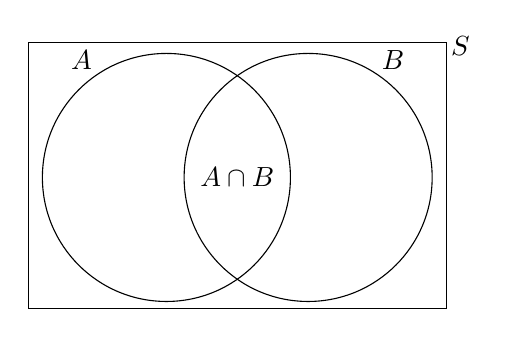
\begin{tikzpicture}[scale=0.9]
				\draw (-2.95, -1.85) rectangle (2.95, 1.9);
				\draw (-1,0) circle (1.75);
				\draw (1,0) circle (1.75);
				\node at (-2.2,1.65) {$A$};
				\node at (2.2,1.65) {$B$};
				\node at (0,0) {$A \cap B$};
				\node at (3.15,1.85) {$S$};
			\end{tikzpicture}
		\end{center}
	\end{frame}


	\begin{frame}{Addition Law of Probability (Three Joint Events)}
		When there are three events:
		\[
		P(A \cup B \cup C) = P(A) + P(B) + P(C) - P(A \cap B) - P(A \cap C) - P(B \cap C) + P(A \cap B \cap C)
		\]

		The above is the probability that at least one or two or all three of the events occur.

	\end{frame}


	\begin{frame}{Addition Law of Probability (Disjoint Case)}
		The addition law gives the probability that at least one of two events occurs.

		\[
		P(A \cup B) = P(A) + P(B)
		\]

		\begin{center}
			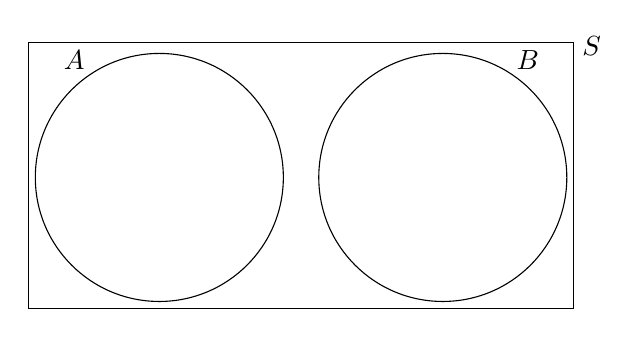
\begin{tikzpicture}[scale=0.9]
				\draw (-3.85, -1.85) rectangle (3.85, 1.9);
				\draw (-2,0) circle (1.75);
				\draw (2,0) circle (1.75);
				\node at (-3.2,1.65) {$A$};
				\node at (3.2,1.65) {$B$};
				\node at (4.1,1.85) {$S$};
			\end{tikzpicture}
		\end{center}

		Here, $P(A \cap B) = 0$ because $A \cap B = \varnothing$
	\end{frame}


	\begin{frame}{Addition Law of Probability (Disjoint Case, More than Two Events)}
		For a sequence of disjoint (mutually exclusive) events $A_1, A_2,...,A_k$:
		\[
			P(A_1, A_2,...,A_k) = P(A_1) + P(A_2) + ... + P(A_k)
		\]
	\end{frame}


	\begin{frame}{Example: Addition Law}
		In a company, $60\%$ of the employees have motorcycle, $40\%$ have private car and $20\%$ have both.
		
		\vspace{0.5em}
		
		If an employee is selected randomly from that company, then
		\begin{enumerate}
			\item What is the probability that the employee has \emph{at least} one type of vehicle?
			\item What is the probability that the employee has \emph{exactly} one type of vehicle?
			\item What is the probability that the employee has neither motorcycle nor private car?
		\end{enumerate}
	\end{frame}


	\begin{frame}{Solution}
		Let,

		$M$ = event that the employee has a motorcycle

		$C$ = event that the employee has a car
		
		\vspace{0.5em}

		Then, $M \cap C$ = event that the employee has both

		\vspace{0.5em}
		Here, $P(M) = 0.6$, $P(C)=0.4$ and $P(M \cap C)=0.2$
	\end{frame}


	\begin{frame}{Solution (cont.)}
		\begin{enumerate}
			\item Probability of having \emph{at least} one type of vehicle:

			$P(M \cup C) = P(M) + P(C) - P(M \cap C) = 0.6 + 0.4 - 0.2 = 0.8$

			\item Probability of having \emph{exactly} one type of vehicle:
			
			$P(M \cup C) - P(M \cap C) = 0.8 - 0.2 = 0.6$

			\item Probability of having neither type of vehicle:
			
			$1 - P(M \cup C) = 1 - 0.8 = 0.2$
		\end{enumerate}
	\end{frame}


	\begin{frame}{Conditional Probability}
		Conditional probability measures the likelihood of an event given that another event has occurred.

		\vspace{0.5em}
		Probability that the event $A$ will occur given that the $B$ has already occurred:
		\[
		P(A \mid B) = \frac{P(A \cap B)}{P(B)}, \quad P(B) > 0
		\]

		Since $B$ has already occurred:
		\begin{itemize}
			\item if the event $A$ is to occur, then the set of favourable outcomes is given by $A \cap B$
			\item it also shrinks the sample space to $B$ only
		\end{itemize}

	\end{frame}


	\begin{frame}{Conditional Probability (cont.)}
		\begin{center}
			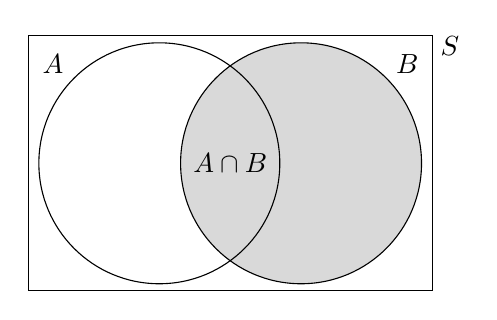
\begin{tikzpicture}[scale=0.9]
				\draw (-2.85, -1.8) rectangle (2.85, 1.8);
				\draw (1,0) circle (1.5);
				\fill[gray!30] (1,0) circle (1.7);
				\draw (1,0) circle (1.7);
				\draw (-1,0) circle (1.7);
				\node at (-2.5,1.4) {$A$};
				\node at (2.5,1.4) {$B$};
				\node at (0,0) {$A \cap B$};
				\node at (3.1,1.65) {$S$};
			\end{tikzpicture}
		\end{center}
		The information that event $B$ has already occured, shrinks the samples space to the set denoted by $B$.
	\end{frame}


	\begin{frame}{Conditional Probability: Example 1}
		The sample space of a dice throw is, $S = \{1, 2, 3, 4, 5, 6\}$, then the probability of getting a $2$ is: $P(2) = 1/6$.

		\vspace{1.5em}

		Suppose it is known that an even number occured (the specific number that occured, is not yet disclosed).
		
		\vspace{0.5em}
		
		Then the sample space shrinks, it becomes: $S^* = \{2, 4, 6\}$. Then $P(2 | \text{even}) = 1/3$.

		\vspace{1.5em}

		It can also be written as: $P(2 | \text{even}) = \frac{P(2 \, \text{and even})}{P(\text{even})} = \frac{1/6}{3/6} = \frac{1}{3}$.
	\end{frame}

	
	\begin{frame}{Conditional Probability: Example 2}
		In a company, $60\%$ of the employees have motorcycle, $40\%$ have private car and $20\%$ have both.
		
		\vspace{0.5em}

		If an employee is selected randomly from that company. What is the probability that:

		\begin{enumerate}
			\item the employee has a car given that he/she has a motorcycle?
			\item the employee has a motorcycle given that he/she has a car?
		\end{enumerate}
	\end{frame}


	\begin{frame}{Conditional Probability: Example 2 Solution}
		\begin{enumerate}
			\item Probability that the employee has a car given that he/she owns a motorcycle:
				\[P(C|M) = \frac{P(C \cap M)}{P(M)} = \frac{0.2}{0.6} = 1/3\]

			\item Probability that the employee has a motorcycle given that he/she owns a car:
				\[P(M|C) = \frac{P(C \cap M)}{P(C)} = \frac{0.2}{0.4} = 1/2\]
		\end{enumerate}
	\end{frame}


	\begin{frame}{Multiplication Law of Probability}
		\begin{itemize}
			\item \textbf{For two \emph{dependent events}} $A$ and $B$, the probability that, both events will occur simultaneously is:
			\[
				P(A \cap B) = P(A)\,P(B \mid A) = P(A \mid B) \, P(B)
			\]

			\item \textbf{For two \emph{independent events}}, the probability of both occuring simultaneously is:
			\[
				P(A \cap B) = P(A)\,P(B)
			\]
		\end{itemize}
	\end{frame}


	\begin{frame}{Multiplication Law of Probability (cont.)}
		Suppose there are three events: $A$, $B$ and $C$.

		Then one of the $3!$ ways to write the multiplication law is:
		\[
			P(A \cap B \cap C) = P(A \mid B \cap C) \, P(B \cap C) = P(A \mid B \cap C) \, P(B \mid C) \, P(C)
		\]
	\end{frame}


	\begin{frame}{Multiplication Law: Example}
		In rainy season, it rains $70\%$ of the days in Bangladesh. When it rains, $80\%$ times it makes thunderstorms.

		\vspace{0.5em}
		
		What is the probability that, in a particular day of rainy season, it will rain and it will thunderstorm?

		\vspace{1.5em}

		Suppose:

		$R$ = event that it rains in that day
		
		$T$ = event that thunderstorm occurs

		\vspace{0.5em}

		Then, $P(R) = 0.7$ and $P(T \mid R) = 0.8$.

		\vspace{0.5em}

		Therefore, $P(T \cap R) = P(T \mid R) \, P(R) = 0.8 \times 0.7 = 0.56$
	\end{frame}


	\begin{frame}{Law of Total Probability}
		Suppose \(B_1, B_2, \dots, B_n\) are mutually exclusive and collectively exhaustive events with \(P(B_i) > 0\). Then for any event \(A\):

		\[
		P(A) = \sum_{i=1}^{n} P(A \mid B_i) P(B_i)
		\]

		The probability of \(A\) is found by breaking the sample space into disjoint parts and weighting conditional probabilities by their proportions.

		\begin{center}
		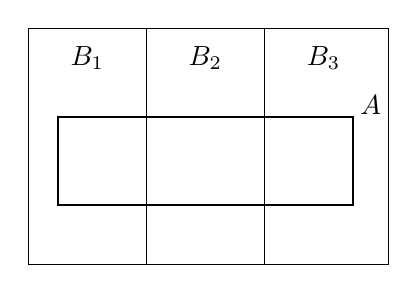
\begin{tikzpicture}[scale=0.75]
			\draw (0,0) rectangle (6.1,4);
			\draw (2,0) -- (2,4);
			\draw (4,0) -- (4,4);
			\node at (1,3.5) {$B_1$};
			\node at (3,3.5) {$B_2$};
			\node at (5,3.5) {$B_3$};
			\draw[thick] (0.5,1) rectangle (5.5,2.5);
			\node at (5.8,2.7) {$A$};
		\end{tikzpicture}
		\end{center}
	\end{frame}


	\begin{frame}{Law of Total Probability: Example}
		A factory has two machines. Machine \(B_1\) produces $60\%$ of items, machine \(B_2\) produces $40\%$. $2\%$ of the items produced by $B_1$ are defective, this rate is $5\%$ for machine $B_2$.

		\vspace{0.5em}
		
		Let $D$ be the event that an item is defective.

		\(P(B_1)=0.6\), \quad \(P(B_2)=0.4\)  

		\(P(D \mid B_1)=0.02\), \quad \(P(D \mid B_2)=0.05\)
		\[
		P(D)=0.02(0.6)+0.05(0.4)=0.012+0.02=0.032
		\]

		Overall probability of a defective item is \(0.032\).
	\end{frame}


	\section*{Thank you.}

\end{document}